\documentclass[11pt,a4paper]{article}
\usepackage[margin=2.5cm]{geometry}
\usepackage{booktabs,graphicx,amsmath,hyperref,float,caption}
\hypersetup{colorlinks=true,linkcolor=black,citecolor=black,urlcolor=blue}
\linespread{1.12}
\graphicspath{{figures/}{./}}
\title{Study-Held-Out Validation of Machine-Learning Models for Biomass Gasification: Random Cross-Validation Overstates Accuracy and Prediction Intervals Remain Wide}
\author{Priom Dey\textsuperscript{*}, Avro Talukder, Yuvraj Roy\\[2pt] \small Department of Chemistry, Shahjalal University of Science and Technology, Sylhet, Bangladesh \\[2pt] \small *Corresponding author: \texttt{2023131044@student.sust.edu} \\ \small ORCID: Priom Dey \href{https://orcid.org/0009-0007-5722-8240}{0009-0007-5722-8240}; Avro Talukder \href{https://orcid.org/0009-0007-6996-7673}{0009-0007-6996-7673} \\ \small Other e-mail addresses: \texttt{2023131055@student.sust.edu} (A.T.);\\ \small \texttt{2023131056@student.sust.edu} (Y.R.)}
\date{}
\begin{document}\sloppy\maketitle

\begin{abstract}
Machine-learning models of biomass gasification are usually tested with random cross-validation, in which experiments from the same publication can appear in both training and test data. We asked how well such models transfer to publications they have not seen. Using an open compilation of 312 gasification experiments from 29 publications (36 differently spelled study names in the file were merged to 29), we predicted gas composition, the share of H$_2$+CO in the nitrogen-free gas (a purity measure), gas yield, gas heating value and cold-gas efficiency from feedstock properties and operating conditions, using random forests, extra trees, gradient boosting and ridge regression.
For the random forest, random five-fold cross-validation gave a skill (reduction in mean absolute error relative to predicting the training mean) of 0.45 to 0.84 across the nine targets, whereas leave-one-publication-out validation gave 0.04 to 0.58; the increase in error was statistically clear for every target (publication-clustered bootstrap). Held-out skill was highest for H$_2$ (0.58), gas heating value (0.53) and H$_2$+CO (0.51); for CO$_2$ and CO the 95\% intervals included zero. A feedstock-class average was no better than the overall average (skill below 0.05).
Conformal prediction intervals calibrated only on training publications had pooled coverage of 0.77 to 0.93 for nominal 80\% and 90\% levels, but were 1.2 to 3.3 standard deviations of the target wide, and every target had at least one publication whose experiments were not covered at all at the 80\% level. Only 9 experiments, all from one publication, were pressurised, so no pressure effect could be learned, and feedstock mixtures are not represented. Accuracy reported with random splits therefore overstates what to expect for a new study or gasifier; we provide a reproducible study-held-out benchmark for this data set.
\end{abstract}
\noindent\textbf{Keywords:} biomass gasification; syngas; machine learning; cross-validation; conformal prediction; uncertainty

\section{Introduction}
Gasification converts biomass and waste into a gas rich in H$_2$ and CO that can be used for heat, power, fuels and chemicals. Its output depends on feedstock composition and on operating conditions such as temperature, equivalence ratio and gasifying agent, and the relations are difficult to model from first principles. Many machine-learning models have therefore been proposed to predict gas composition, yield and efficiency from these inputs \cite{Ascher2022review}.

Most such studies assemble experiments from many publications and then evaluate the model with random train/test splits or random cross-validation. Experiments from one publication share a gasifier, a feedstock batch and a measurement protocol, so a random split lets the model see closely related experiments during training. This is the kind of structure for which random cross-validation is known to give optimistic estimates \cite{Roberts2017}, and generalisation to new chemistry or conditions can be much worse than the random-split error suggests \cite{Meredig2018}. A user who wants to predict a new gasifier or a new study, however, needs exactly that second quantity.
The open data set of Ascher et al.\ \cite{Ascher2022}, which compiles gasification experiments from the literature together with the publication each comes from, makes it possible to measure it. To the best of our reading of the code released with that data set, the models there were evaluated with random repeated $k$-fold and train/test splits and the publication of each experiment was not used for grouping.

This study therefore asks five questions on that data set with free software: (i) how much does accuracy fall when whole publications are withheld instead of random experiments; (ii) for which outputs, including a purity measure of the syngas, is the held-out skill clearly better than simply predicting the training mean; (iii) do conformal prediction intervals calibrated on other publications keep their nominal coverage on a new publication, and how wide are they; (iv) how do the results differ between feedstock classes; and (v) what can be said about pressure, which is often named as a key operating variable. We do not claim better models; we aim to show what the data can and cannot support.

\section{Data and Methods}
\subsection{Data}
We used the open compilation of Ascher et al.\ \cite{Ascher2022} (sheet ``Clean Data'', repository commit \texttt{b4b7505}), which contains 312 experiments with feedstock ultimate and proximate analysis, feedstock class, operating conditions, reactor descriptors, gas composition (vol.\% dry basis), gas yield, gas lower heating value (LHV) and cold-gas efficiency (CGE). The notebook downloads the original file and does not redistribute it. The file names the source of each experiment, but the same publication is sometimes spelled differently (a trailing space, a misspelled author name, or different end-page numbers). The file contains 36 distinct study names; after merging spelling variants (affecting several publications) we obtained 29 publications. Without this correction, parts of one publication could fall on both sides of a held-out split. Feedstock classes in the file are woody biomass (166 experiments), herbaceous biomass (57), municipal solid waste (31), sewage sludge (23), plastics (21) and other (14). Herbaceous biomass is the class that corresponds most closely to agricultural residues, but the file does not separate agricultural residues from other herbaceous material, and it contains no information on mixtures of feedstocks.

\subsection{Targets and inputs}
The nine targets were the volume fractions of H$_2$, CO, CO$_2$ and CH$_4$ (vol.\% dry basis, including N$_2$ dilution), their sum H$_2$+CO, the \emph{N$_2$-free syngas share} $100(\mathrm{H_2}+\mathrm{CO})/(\mathrm{H_2}+\mathrm{CO}+\mathrm{CO_2}+\mathrm{CH_4})$, which we use as a purity measure that does not depend on how much air was used, gas yield (Nm$^3$/kg), gas LHV (MJ/Nm$^3$) and CGE (\%). Fifteen experiments with a reported CGE above 100\% are physically impossible and were removed from the CGE target only, leaving 263 experiments. Numbers of experiments per target are in Table~\ref{tab:main}.
Inputs were the feedstock ultimate analysis (C, H, N, S, O), lower heating value, particle size, ash and moisture, temperature, equivalence ratio, an indicator for pressurised operation, and categorical descriptors (feedstock class, gasifying agent, reactor type, operating mode, catalyst, scale, bed material). Residence time and steam-to-biomass ratio were dropped because more than half of their values are missing; the gasifying agent partly carries the steam information. Pressure is given as a number (205~kPa) for only 9 experiments; all others are ``atmospheric'', ``slightly above/below atmospheric'' or blank, so we used a single indicator (pressure above 150~kPa) rather than inventing numeric values. Missing numeric values were filled with the training median and a missing-value indicator was added; rare categories (fewer than five training experiments) were pooled. All preprocessing was fitted inside each training fold.

\subsection{Models}
We compared ridge regression, random forests (200 trees, half the features per split, minimum leaf size 2) \cite{Breiman2001}, extra trees (same settings) \cite{Geurts2006} and histogram gradient boosting (150 iterations, learning rate 0.05, depth 3) from \texttt{scikit-learn} \cite{Pedregosa2011}. Two baselines were the training mean and the mean of the training experiments of the same feedstock class. No hyperparameters were tuned; the settings were fixed before the analysis.

\subsection{Validation protocols and statistics}
\emph{Random} validation used five-fold cross-validation repeated three times with different shuffles. \emph{Study-held-out} validation left out all experiments of one publication at a time (leave-one-publication-out) and trained on the others. Errors are pooled out-of-fold predictions. We report the mean absolute error (MAE) and $R^2$ and the \emph{skill} $=1-\mathrm{MAE}/\mathrm{MAE}_{\text{mean}}$, where $\mathrm{MAE}_{\text{mean}}$ is the error of predicting the training mean under the same protocol; skill 0 means no better than the mean and 1 means no error. The 95\% intervals come from a bootstrap that resamples whole publications ($2000$ resamples), and the same resamples are used for the paired comparison of protocols and of models.

\subsection{Prediction intervals}
For the random forest we built split-conformal intervals \cite{Lei2018,Angelopoulos2023}. For each held-out publication, absolute residuals were obtained by an inner grouped five-fold cross-validation (100 trees) over the \emph{training} publications only, and the interval half-width was the finite-sample-corrected quantile of these residuals for the nominal level (80\% and 90\%). The held-out publication therefore never influenced its own interval. We report the pooled fraction of held-out experiments inside the interval, the fraction of publications with coverage below nominal, and the interval width relative to the standard deviation of the target.

\subsection{Feature importance}
Permutation importance was computed on held-out publications: each input was shuffled within each held-out fold (three shuffles) and the increase in pooled squared error relative to the unshuffled error was recorded. Importance describes what the fitted models use, not causal effects, and is shared among correlated inputs.

\section{Results}
\subsection{Random versus study-held-out validation}
Table~\ref{tab:main} and Fig.~\ref{fig:skill} compare the two protocols for the random forest. With random cross-validation the skill was 0.45 to 0.84 across the nine targets; with leave-one-publication-out validation it was 0.04 to 0.58. The mean absolute error was higher under study-held-out validation for every target, and the 95\% interval of the increase excluded zero in every case (Table~\ref{tab:main}). The held-out skill was clearly above zero (95\% interval above zero) for H$_2$, CH$_4$, H$_2$+CO, N$_2$-free syngas share, gas yield, gas LHV, and CGE (for CGE the lower limit is only just above zero); for CO and CO$_2$ the interval included zero, so we cannot show that the model is better than predicting the training mean for a new publication. Fig.~\ref{fig:parity} shows the held-out predictions: groups of experiments from the same publication are often displaced together from the diagonal, which is the typical signature of study-level offsets that a random split would hide.

\begin{table}[H]\centering\footnotesize\setlength{\tabcolsep}{3pt}\caption{Random forest: random five-fold (3 repeats) versus leave-one-publication-out validation. $n$ experiments from $N$ publications. MAE in the unit of the target; intervals are 95\% bootstrap intervals over publications. Skill $=1-\mathrm{MAE}/\mathrm{MAE}_{\text{mean}}$.}\label{tab:main}
\resizebox{\linewidth}{!}{\begin{tabular}{lcccccccc}\toprule
Target & $n$ & $N$ & MAE random & MAE held-out [95\% CI] & Increase [95\% CI] & Skill random & Skill held-out [95\% CI] & $R^2$ held-out\\\midrule
H$_2$ (vol.\%) & 312 & 29 & 2.93 & 6.13 [4.41, 8.42] & 3.20 [1.79, 5.36] & 0.79 & 0.58 [0.38, 0.71] & 0.76 \\
CO (vol.\%) & 309 & 29 & 2.61 & 6.39 [4.89, 7.90] & 3.78 [2.37, 5.21] & 0.65 & 0.17 [-0.03, 0.31] & 0.18 \\
CO$_2$ (vol.\%) & 309 & 29 & 1.73 & 4.62 [3.19, 6.24] & 2.89 [1.41, 4.57] & 0.63 & 0.04 [-0.11, 0.14] & -0.00 \\
CH$_4$ (vol.\%) & 309 & 29 & 0.942 & 2.04 [1.62, 2.42] & 1.10 [0.78, 1.42] & 0.67 & 0.30 [0.15, 0.45] & 0.35 \\
H$_2$+CO (vol.\%) & 309 & 29 & 3.16 & 9.91 [6.82, 14.21] & 6.75 [3.62, 11.23] & 0.84 & 0.51 [0.32, 0.67] & 0.59 \\
H$_2$+CO share of N$_2$-free gas (\%) & 309 & 29 & 3.31 & 8.92 [6.61, 11.41] & 5.61 [3.61, 7.54] & 0.70 & 0.21 [0.04, 0.37] & 0.21 \\
gas yield (Nm$^3$/kg) & 278 & 26 & 0.210 & 0.485 [0.275, 0.772] & 0.275 [0.089, 0.511] & 0.67 & 0.28 [0.15, 0.44] & 0.30 \\
gas LHV (MJ/Nm$^3$) & 312 & 29 & 0.538 & 1.49 [1.02, 2.08] & 0.948 [0.506, 1.565] & 0.82 & 0.53 [0.35, 0.67] & 0.66 \\
cold-gas efficiency (\%) & 263 & 26 & 7.82 & 12.58 [10.64, 14.62] & 4.77 [2.98, 6.52] & 0.45 & 0.14 [0.00, 0.26] & 0.21 \\
\bottomrule\end{tabular}}\end{table}

\begin{figure}[H]\centering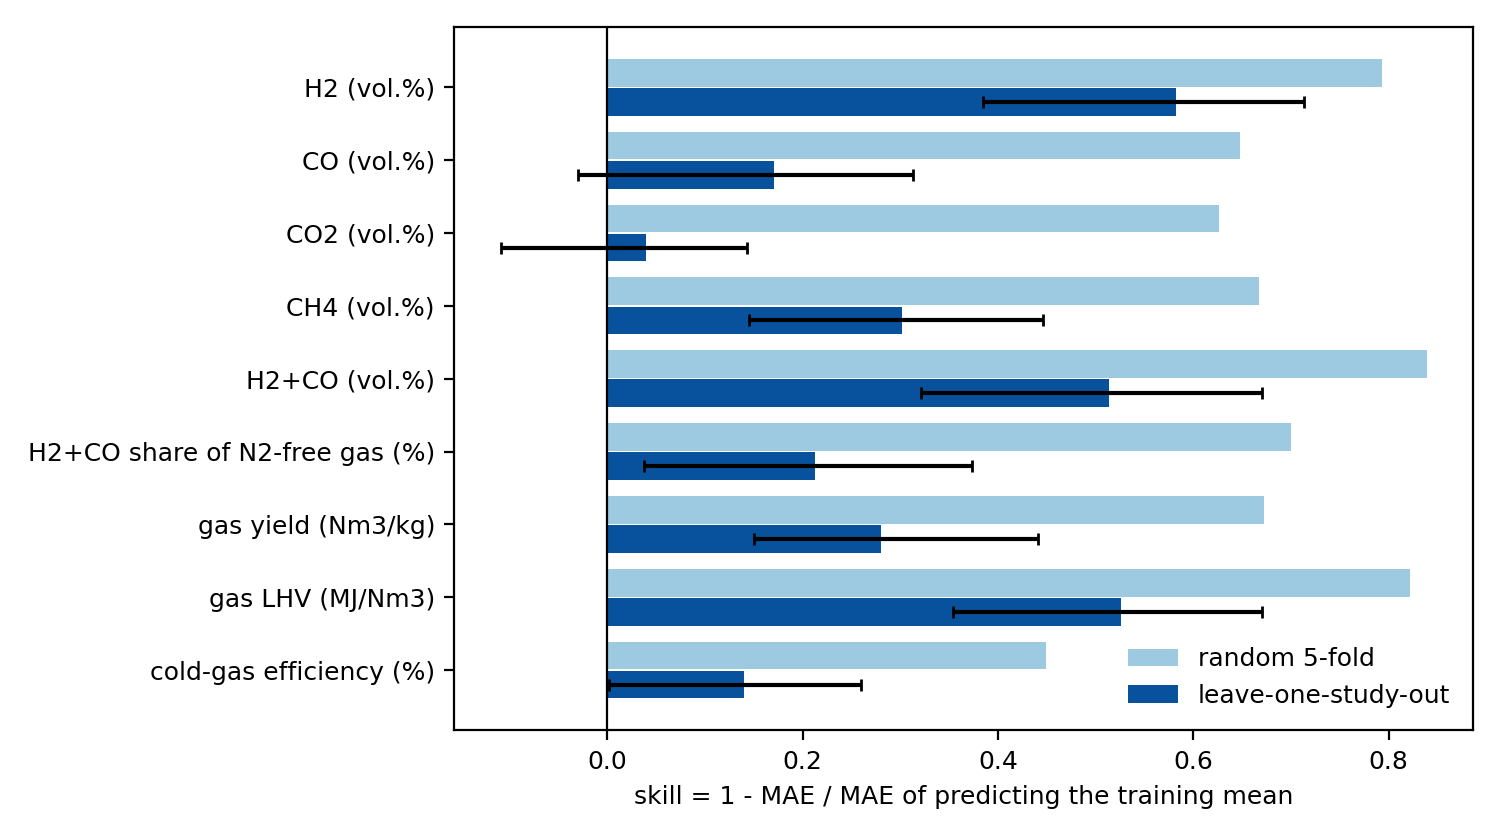
\includegraphics[width=.8\linewidth]{fig1_skill_random_vs_study.png}\caption{Skill of the random forest under random five-fold and leave-one-publication-out validation (error bars: 95\% bootstrap interval over publications).}\label{fig:skill}\end{figure}
\begin{figure}[H]\centering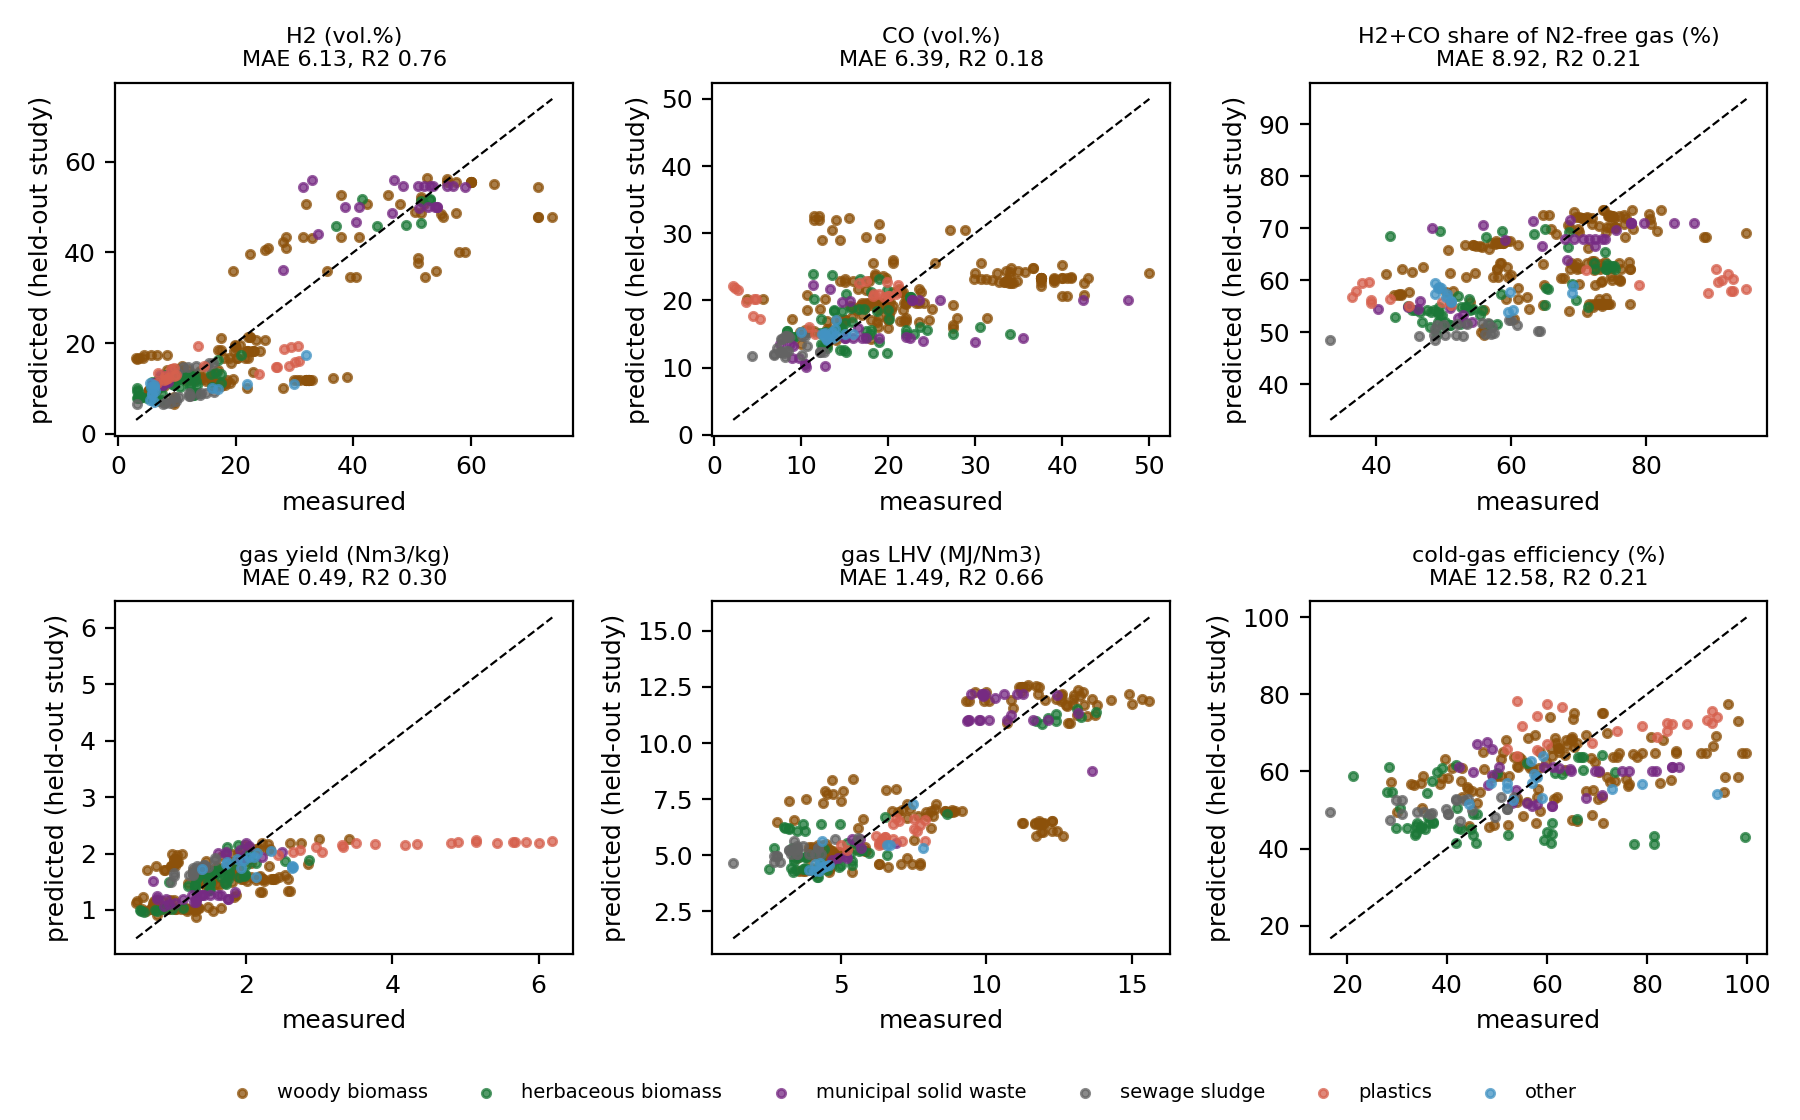
\includegraphics[width=.95\linewidth]{fig2_parity_study_held_out.png}\caption{Held-out predictions of the random forest, coloured by feedstock class.}\label{fig:parity}\end{figure}

\subsection{Comparison of models}
Table~\ref{tab:models} gives the held-out MAE of all models. A feedstock-class average was no better than the overall average (skill at most 0.04), so the feedstock label alone carries almost no transferable information. Among the learned models there was no single winner: the random forest had the lowest held-out MAE for 4 of the nine targets, and gradient boosting, extra trees and ridge regression were best for the others (bold in Table~\ref{tab:models}). Ridge regression was worse than the training mean for CH$_4$, CO, CO$_2$ and CGE, but gave the lowest error for gas yield. Differences among the three tree ensembles were small compared with the differences between protocols, and we did not tune any model, so these rankings should not be over-interpreted.

\begin{table}[H]\centering\footnotesize\caption{Held-out MAE (leave-one-publication-out) of all models; bold = lowest among the four learned models.}\label{tab:models}
\resizebox{\linewidth}{!}{\begin{tabular}{lcccccc}\toprule
Target & Training mean & Feedstock-class mean & Ridge & Random forest & Extra trees & Grad.\ boosting\\\midrule
H$_2$ (vol.\%) & 14.67 & 14.68 & 10.29 & \textbf{6.13} & 6.82 & 6.83 \\
CO (vol.\%) & 7.70 & 7.76 & 10.79 & \textbf{6.39} & 6.73 & 6.60 \\
CO$_2$ (vol.\%) & 4.81 & 4.93 & 5.02 & 4.62 & \textbf{4.62} & 4.73 \\
CH$_4$ (vol.\%) & 2.92 & 2.89 & 3.28 & \textbf{2.04} & 2.19 & 2.32 \\
H$_2$+CO (vol.\%) & 20.40 & 19.91 & 13.87 & \textbf{9.91} & 10.25 & 10.18 \\
H$_2$+CO share of N$_2$-free gas (\%) & 11.33 & 11.14 & 9.74 & 8.92 & \textbf{7.64} & 9.26 \\
gas yield (Nm$^3$/kg) & 0.674 & 0.670 & \textbf{0.428} & 0.485 & 0.492 & 0.558 \\
gas LHV (MJ/Nm$^3$) & 3.14 & 3.01 & 2.02 & 1.49 & 1.63 & \textbf{1.37} \\
cold-gas efficiency (\%) & 14.63 & 14.91 & 15.09 & 12.58 & 13.84 & \textbf{12.12} \\
\bottomrule\end{tabular}}\end{table}

\subsection{Prediction intervals for new publications}
Table~\ref{tab:conf} and Fig.~\ref{fig:conf} give the conformal results for six targets. Pooled over all held-out experiments the coverage was 0.77 to 0.81 for the nominal 80\% level and 0.86 to 0.93 for 90\%, close to nominal. The intervals were, however, wide: their full width was 1.2 to 3.3 times the standard deviation of the target, so they exclude only a small part of the range of the data for CO and CGE. Coverage also differed greatly between publications: for every target at least one publication had no experiment inside the 80\% interval, and between 15\% and 38\% of publications were below the nominal 80\% coverage. Pooled coverage thus hides the fact that a particular new study can lie entirely outside the interval.

\begin{table}[H]\centering\footnotesize\setlength{\tabcolsep}{4pt}\caption{Conformal prediction intervals for new publications (random forest). Coverage is pooled over held-out experiments; width is the full interval width divided by the standard deviation of the target; the last two columns give the share of publications whose own coverage was below nominal.}\label{tab:conf}
\resizebox{\linewidth}{!}{\begin{tabular}{lcccccc}\toprule
Target & Coverage (80\%) & Coverage (90\%) & Width/SD (80\%) & Width/SD (90\%) & Below nominal (80\%) & Below nominal (90\%)\\\midrule
H$_2$ (vol.\%) & 0.81 & 0.89 & 1.2 & 1.8 & 28\% & 24\% \\
CO (vol.\%) & 0.77 & 0.91 & 2.2 & 3.3 & 38\% & 28\% \\
H$_2$+CO (vol.\%) & 0.81 & 0.93 & 1.4 & 2.0 & 24\% & 7\% \\
H$_2$+CO share of N$_2$-free gas (\%) & 0.81 & 0.88 & 2.3 & 2.8 & 21\% & 14\% \\
gas yield (Nm$^3$/kg) & 0.80 & 0.86 & 1.5 & 2.0 & 15\% & 19\% \\
cold-gas efficiency (\%) & 0.80 & 0.92 & 2.2 & 2.9 & 38\% & 23\% \\
\bottomrule\end{tabular}}\end{table}
\begin{figure}[H]\centering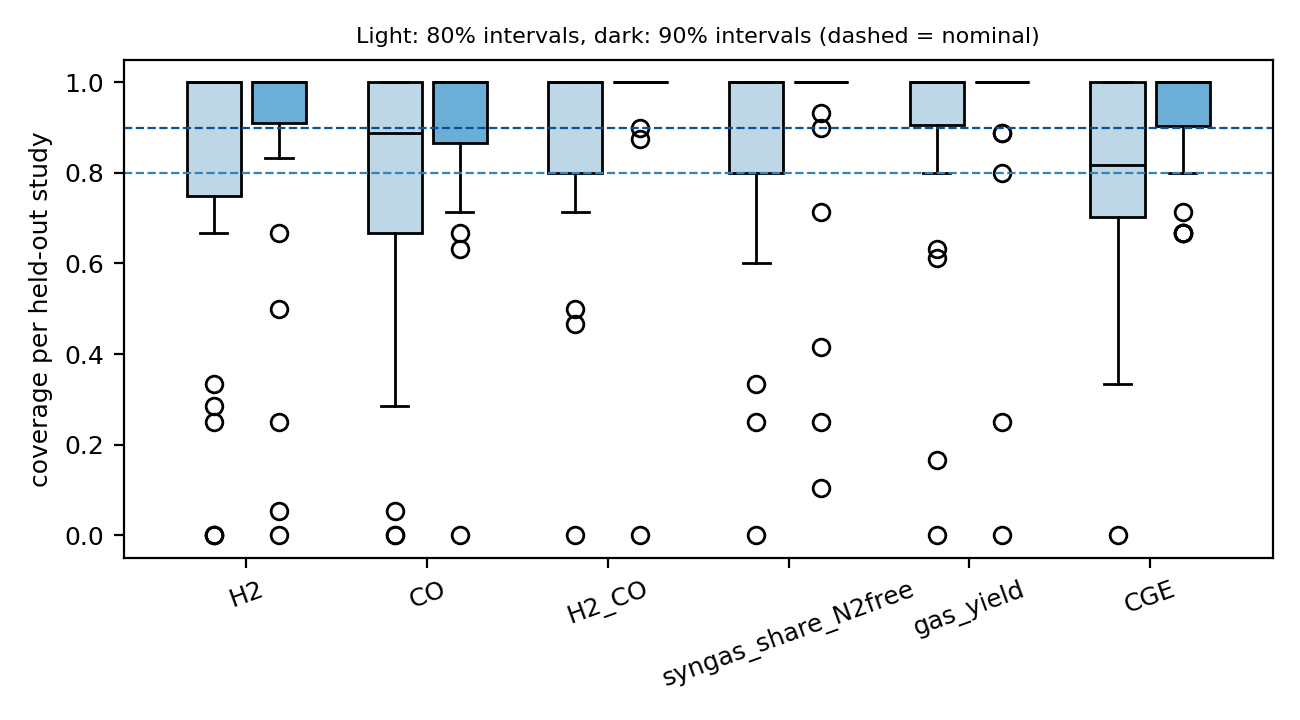
\includegraphics[width=.75\linewidth]{fig3_conformal_coverage_by_study.png}\caption{Coverage of the conformal intervals for each held-out publication (box plots over publications; dashed lines: nominal levels).}\label{fig:conf}\end{figure}

\subsection{Feedstock classes}
Table~\ref{tab:feed} shows the held-out skill by feedstock class. For H$_2$ the skill was 0.78 for herbaceous biomass and 0.47 for woody biomass, but for CO it was only 0.09 and 0.08, respectively. Sewage sludge and plastics each come from a single publication, so the model had no experiment of the same class in training when these were held out; results for them are extrapolation and should not be generalised. Classes with few publications (municipal solid waste, other) have wide uncertainty that is not shown in the table.

\begin{table}[H]\centering\footnotesize\caption{Held-out skill of the random forest by feedstock class ($n$ experiments, $N$ publications for H$_2$; $n$ differs slightly for other targets).}\label{tab:feed}
\resizebox{\linewidth}{!}{\begin{tabular}{lccccccc}\toprule
Feedstock class & $n$ & $N$ & H$_2$ & CO & H$_2$+CO & gas yield & CGE\\\midrule
woody biomass & 166 & 20 & 0.47 & 0.08 & 0.42 & 0.28 & 0.07 \\
herbaceous biomass & 57 & 9 & 0.78 & 0.09 & 0.61 & 0.46 & 0.18 \\
municipal solid waste & 31 & 4 & 0.74 & 0.19 & 0.75 & 0.42 & -0.10 \\
sewage sludge & 23 & 1 & 0.76 & 0.62 & 0.63 & 0.18 & 0.46 \\
plastics & 21 & 1 & 0.25 & -0.01 & 0.19 & 0.22 & 0.20 \\
other & 14 & 2 & 0.52 & 0.71 & 0.66 & 0.16 & -0.01 \\
\bottomrule\end{tabular}}\end{table}

\subsection{Pressure}
Only 9 of the 312 experiments are pressurised (205~kPa), and all of them belong to one publication. When this publication was held out, the model had never seen a pressurised experiment, so the results in Table~\ref{tab:press} describe extrapolation from atmospheric data and say nothing about how pressure changes the output. The held-out skill for the pressurised experiments was similar to the others for H$_2$ but negative for CO, which with nine experiments from one source is not evidence of a pressure effect. A model of the effect of pressure on gasification cannot be built from this data set.

\begin{table}[H]\centering\footnotesize\caption{Held-out error of the random forest for pressurised and other experiments (leave-one-publication-out). Gas yield and CGE have no pressurised experiments in the data.}\label{tab:press}
\resizebox{\linewidth}{!}{\begin{tabular}{llcccccc}\toprule
Target & Subset & $n$ & $N$ & MAE (RF) & MAE (training mean) & Skill\\\midrule
H$_2$ & pressurised ($>$150~kPa) & 9 & 1 & 3.50 & 7.57 & 0.54 \\
H$_2$ & all other & 303 & 28 & 6.21 & 14.88 & 0.58 \\
CO & pressurised ($>$150~kPa) & 9 & 1 & 6.03 & 5.57 & -0.08 \\
CO & all other & 300 & 28 & 6.40 & 7.77 & 0.18 \\
gas yield & all other & 278 & 26 & 0.485 & 0.674 & 0.28 \\
CGE & all other & 263 & 26 & 12.58 & 14.63 & 0.14 \\
\bottomrule\end{tabular}}\end{table}

\subsection{Which inputs matter}
Table~\ref{tab:imp} lists the three inputs with the largest permutation importance on held-out publications (Fig.~\ref{fig:imp}). For H$_2$ the gasifying agent was by far the most important input (0.188), followed by equivalence ratio and temperature; for CGE temperature and ash content; for gas yield ash content, equivalence ratio and temperature. For CO no input had a held-out importance above 0.01, consistent with its low skill. These importances describe the fitted models on held-out publications and are not causal effects.

\begin{table}[H]\centering\footnotesize\caption{Largest permutation importances on held-out publications (increase in squared error relative to unshuffled; random forest).}\label{tab:imp}
\resizebox{\linewidth}{!}{\begin{tabular}{ll}\toprule
Target & Three largest importances\\\midrule
H$_2$ & gasifying agent (0.188); equivalence ratio (0.054); temperature (0.022) \\
CO & particle size (0.004); feedstock C (0.003); feedstock O (0.002) \\
gas yield & ash content (0.021); equivalence ratio (0.019); temperature (0.015) \\
CGE & temperature (0.049); ash content (0.030); feedstock H (0.014) \\
\bottomrule\end{tabular}}\end{table}
\begin{figure}[H]\centering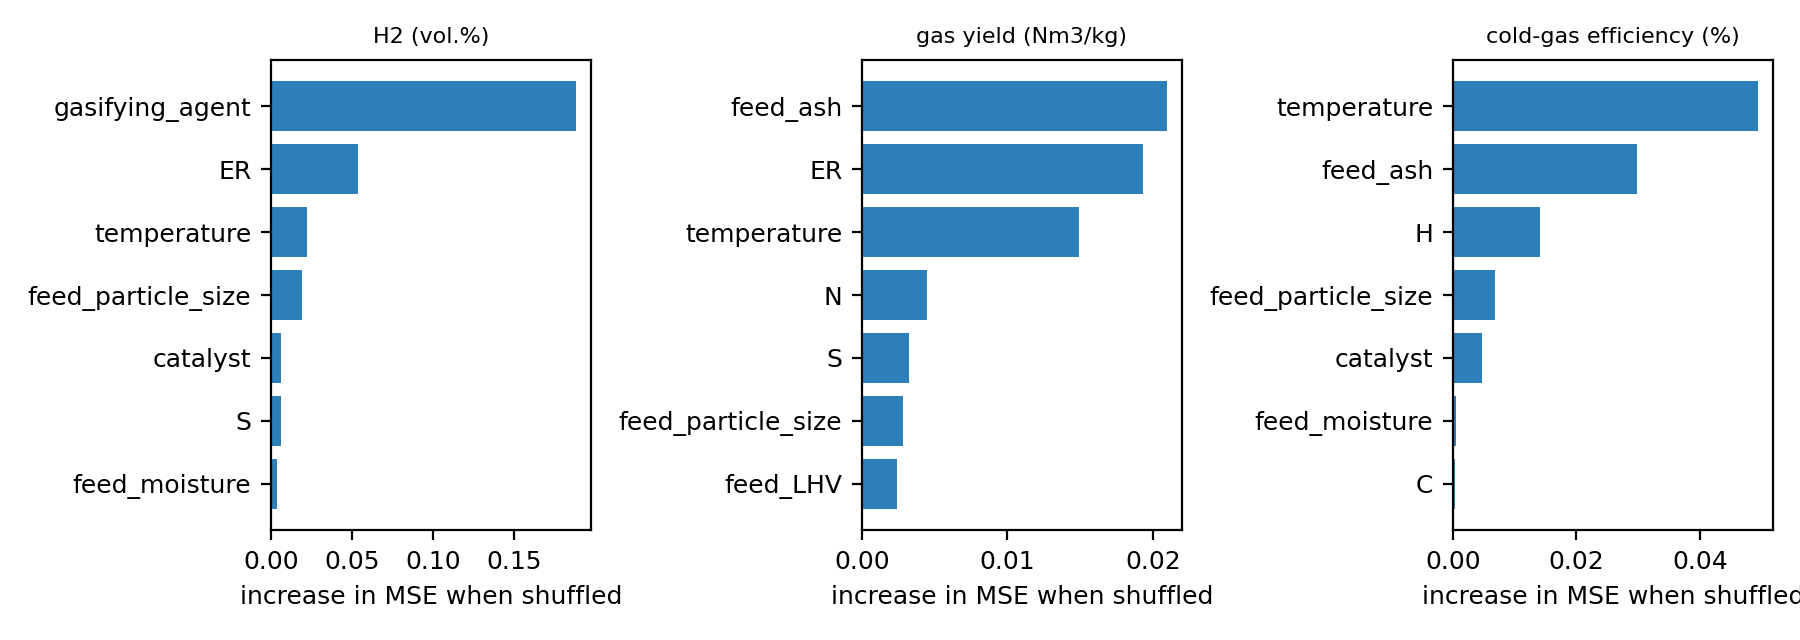
\includegraphics[width=.95\linewidth]{fig4_permutation_importance.png}\caption{Permutation importance on held-out publications for three targets (random forest).}\label{fig:imp}\end{figure}

\section{Discussion}
The central result is the size of the gap between random and study-held-out validation: for every target the error was clearly higher for a publication the model had not seen, and for CO and CO$_2$ the model was not distinguishable from predicting the training mean. The explanation is plausible but is not tested here: each publication has its own gasifier, feedstock batch and measurement practice, and these study-level effects cannot be inferred from the inputs available in the data set. The practical consequence is that accuracy figures from random splits, which are common in this field, should not be used to judge how a model will perform for a new reactor or a new laboratory; leave-one-publication-out error is the more relevant figure, and it should be reported with its interval.

The outputs that transferred best (H$_2$, H$_2$+CO and gas LHV) are those that depend strongly on the gasifying agent and equivalence ratio, which are well represented in the data; the outputs that transferred worst (CO, CO$_2$) are smaller fractions that depend on details of the reactor and on the water--gas shift and are not captured by the inputs. The conformal intervals show the cost of this: they are valid on average over publications, but wide, and a single new publication can lie entirely outside them. We therefore advise against using point predictions, or intervals of this kind, for design decisions on a new gasifier without local data.

The data set also limits what can be asked. The user-facing questions that motivated this work, namely predictions for mixtures of agricultural wastes and for the effect of pressure, cannot be answered: no mixtures are labelled, and the only pressurised experiments come from one publication. Collecting systematically varied pressure and mixture experiments, and publishing them with a clear study identifier, would add more than any further modelling of the present data.

\paragraph{Limitations.}
(i) The data are a literature compilation with unit conversions and assumptions made by its authors, and some values are inconsistent (we removed 15 impossible CGE values and merged spelling variants of study names; other errors may remain). (ii) The data come from 29 publications, so intervals for publication-level quantities are wide; plastics and sewage sludge come from one publication each. (iii) Residence time and steam-to-biomass ratio had to be dropped because of missing values, and pressure could be represented only by a single indicator. (iv) We did not tune the models, so absolute errors are not the best attainable; the conclusions about the protocols concern the gap between them. (v) The conformal procedure assumes that publications are exchangeable, which does not hold for imbalanced feedstock classes. (vi) Results depend slightly on the computing environment; an independent re-run in a different environment gave errors within about 1\% of those reported.

\section{Conclusions}
Using an open compilation of gasification experiments, random cross-validation overstated the skill of machine-learning models relative to validation on unseen publications for all nine outputs, with held-out skill of 0.04 to 0.58 against 0.45 to 0.84 under random folds. H$_2$, H$_2$+CO and gas heating value transferred reasonably, whereas CO and CO$_2$ could not be shown to be better than the training mean. Prediction intervals calibrated on other publications had near-nominal pooled coverage but were wide and failed completely for some publications. Pressure and feedstock mixtures cannot be studied with the current data. We recommend that gasification models be validated by leave-one-publication-out and that data be published with a study identifier.

\section*{Data and Code Availability}
The experimental data are the public data set of Ascher et al.\ \cite{Ascher2022}; please cite that work when using it. The analysis notebook, the result tables and figures, and the script that generates this manuscript are openly available on GitHub and archived on Zenodo (\href{https://doi.org/10.5281/zenodo.23645766}{doi:10.5281/zenodo.23645766}); the Ascher et al.\ data are not redistributed and are downloaded from the original source by the notebook. The results reported here come from \texttt{scikit-learn} 1.6.1 run in Google Colab.

\section*{Author Contributions}
\textbf{Priom Dey:} conceptualization, methodology, software, formal analysis, investigation, data curation, validation, visualization, writing -- original draft, writing -- review and editing. \textbf{Avro Talukder} and \textbf{Yuvraj Roy:} validation (checking of cited sources and of reported numbers against the supplied tables), writing -- review and editing.

\section*{Declaration of AI Assistance}
Generative AI (Anthropic's Claude) was used to help write the analysis code and to draft and edit the manuscript. The corresponding author ran the notebook; all authors reviewed the manuscript, and the authors take full responsibility for the content. AI tools are not listed as authors.

\section*{Funding}
This research received no specific grant from any funding agency in the public, commercial or not-for-profit sectors.

\section*{Competing Interests}
The authors declare no competing interests.

\begin{thebibliography}{99}\small
\bibitem{Ascher2022} S.~Ascher, X.~Wang, I.~Watson, W.~Sloan, S.~You, Interpretable machine learning to model biomass and waste gasification, \emph{Bioresour.\ Technol.} \textbf{364}, 128062 (2022). doi:10.1016/j.biortech.2022.128062
\bibitem{Ascher2022review} S.~Ascher, I.~Watson, S.~You, Machine learning methods for modelling the gasification and pyrolysis of biomass and waste, \emph{Renew.\ Sustain.\ Energy Rev.} \textbf{155}, 111902 (2022). doi:10.1016/j.rser.2021.111902
\bibitem{Roberts2017} D.~R.~Roberts et al., Cross-validation strategies for data with temporal, spatial, hierarchical, or phylogenetic structure, \emph{Ecography} \textbf{40}, 913--929 (2017).
\bibitem{Meredig2018} B.~Meredig et al., Can machine learning identify the next high-temperature superconductor? Examining extrapolation performance for materials discovery, \emph{Mol.\ Syst.\ Des.\ Eng.} \textbf{3}, 819--825 (2018). doi:10.1039/C8ME00012C
\bibitem{Breiman2001} L.~Breiman, Random forests, \emph{Mach.\ Learn.} \textbf{45}, 5 (2001).
\bibitem{Geurts2006} P.~Geurts, D.~Ernst, L.~Wehenkel, Extremely randomized trees, \emph{Mach.\ Learn.} \textbf{63}, 3 (2006).
\bibitem{Pedregosa2011} F.~Pedregosa et al., Scikit-learn: machine learning in Python, \emph{J.\ Mach.\ Learn.\ Res.} \textbf{12}, 2825 (2011).
\bibitem{Lei2018} J.~Lei, M.~G'Sell, A.~Rinaldo, R.~J.~Tibshirani, L.~Wasserman, Distribution-free predictive inference for regression, \emph{J.\ Am.\ Stat.\ Assoc.} \textbf{113}, 1094 (2018). doi:10.1080/01621459.2017.1307116
\bibitem{Angelopoulos2023} A.~N.~Angelopoulos, S.~Bates, Conformal prediction: a gentle introduction, \emph{Found.\ Trends Mach.\ Learn.} \textbf{16}, 494--591 (2023). doi:10.1561/2200000101
\end{thebibliography}
\end{document}
